\documentclass[12pt,letterpaper,onecolumn]{exam}
\usepackage{amsmath,amsfonts,amssymb,amsthm}
\usepackage{graphicx}
\usepackage[lmargin=71pt,tmargin=1in]{geometry}

\begin{document}
\thispagestyle{empty}
\begingroup
    \centering
    \LARGE Machine Learning\\
    \LARGE Homework 3\\[0.5em]
    \normalsize Released: Nov. 24, 2026 \qquad Due: Dec. 16, 2026\\[0.5em]
    \large Fill your Name \qquad Fill your Student ID\par
\endgroup
\noindent\rule{\textwidth}{0.4pt}\par
\printanswers
\renewcommand{\solutiontitle}{\noindent\textbf{Ans:}\enspace}

\begin{questions}
    \question
    Consider a neural network with $d$ inputs, $n$ hidden neurons, and
    $q$ outputs, as shown in Figure~\ref{fig:network},
    where $d,n\geq 1$ and $q\geq 2$.

    \begin{figure}[ht]
        \centering
        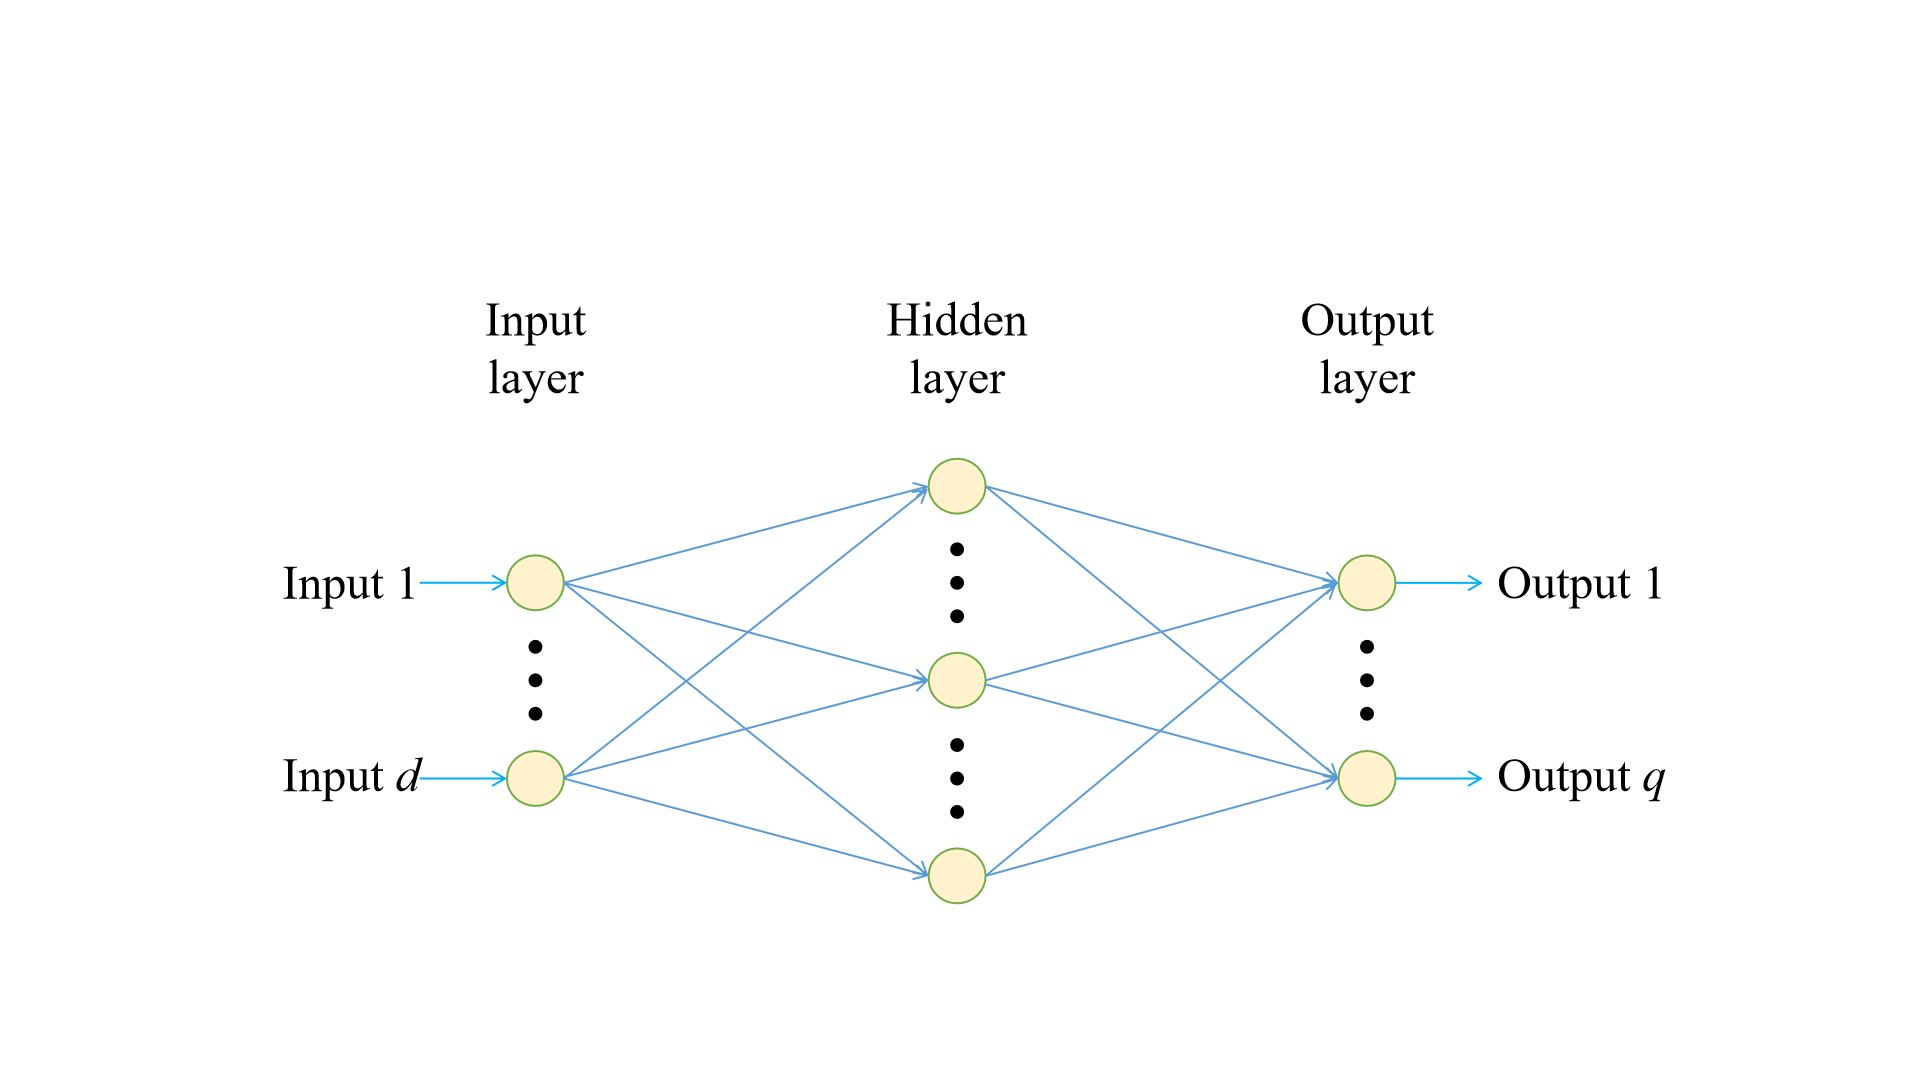
\includegraphics[width=0.78\linewidth,
            trim=175bp 90bp 165bp 195bp,clip]{network.png}
        \caption{A fully connected network with one hidden layer.}
        \label{fig:network}
    \end{figure}

    All vectors are column vectors. The parameters are
    \[
        W^1\in\mathbb{R}^{d\times n},\quad b^1\in\mathbb{R}^n,
        \qquad W^2\in\mathbb{R}^{n\times q},\quad b^2\in\mathbb{R}^q.
    \]
    For one input $x\in\mathbb{R}^d$, the forward propagation is
    \[
        z^1=(W^1)^Tx+b^1,\qquad h=\sigma(z^1),\qquad
        z^2=(W^2)^Th+b^2,\qquad \hat y=\operatorname{Softmax}(z^2),
    \]
    where $\sigma(u)=1/(1+e^{-u})$ acts element-wise and
    $\hat y_k=e^{z^2_k}/\sum_{j=1}^q e^{z^2_j}$.
    Let $y\in\{0,1\}^q$ be a one-hot target, so $\sum_{k=1}^q y_k=1$.
    Define the cross-entropy loss and the regularized objective by
    \begin{equation}
        L_{\mathrm{CE}}=-\sum_{k=1}^q y_k\log\hat y_k,
        \qquad
        J=L_{\mathrm{CE}}+
        \frac{\lambda}{2}\left(\|W^1\|_F^2+\|W^2\|_F^2\right).
    \end{equation}
    Here $\lambda>0$ is given, $\|W\|_F^2=\sum_{i,j}W_{ij}^2$,
    and the biases are not regularized. The logarithm is natural.
    Show intermediate chain-rule steps and state the dimensions of
    all vector and matrix gradients.
    \begin{parts}
        \part Derive $\delta^2=\partial L_{\mathrm{CE}}/\partial z^2$.
        Show how the softmax and cross-entropy derivatives simplify.
        \part Derive $\partial J/\partial W^2$ and
        $\partial J/\partial b^2$. Then derive
        $\delta^1=\partial L_{\mathrm{CE}}/\partial z^1$ and obtain
        $\partial J/\partial W^1$ and $\partial J/\partial b^1$.
        \part Write the gradient descent updates for $W^1$ and $W^2$
        with learning rate $\eta>0$. Explain how regularization changes
        these updates compared with $\lambda=0$.
    \end{parts}
    \textit{Hint:} $\sigma'(u)=\sigma(u)(1-\sigma(u))$.
    You may use $\odot$ for element-wise multiplication.

    \begin{solution}
        \begin{parts}
            \part
            \part
            \part
        \end{parts}
    \end{solution}

    \newpage
    \question
    Use the same matrix convention as in Problem 1, but replace the
    hidden activation by $\operatorname{ReLU}(u)=\max\{0,u\}$,
    applied element-wise, and set $\lambda=0$ (no regularization).
    The output activation is still softmax, and the loss is
    $L_{\mathrm{CE}}$. Let $d=n=q=2$ and
    \[
        x=\begin{bmatrix}1\\-1\end{bmatrix},\qquad
        y=\begin{bmatrix}0\\1\end{bmatrix}.
    \]
    The initial parameters are
    \[
        W^1=\begin{bmatrix}0.4&-0.3\\0.2&0.5\end{bmatrix},
        \qquad b^1=\begin{bmatrix}0.1\\0.2\end{bmatrix},
    \]
    \[
        W^2=\begin{bmatrix}0.6&-0.4\\-0.2&0.3\end{bmatrix},
        \qquad b^2=\begin{bmatrix}0.1\\-0.1\end{bmatrix}.
    \]
    \begin{parts}
        \part Perform forward propagation. Compute $z^1$, $h$, $z^2$,
        $\hat y$, and $L_{\mathrm{CE}}$.
        \part Perform backpropagation. Compute $\delta^2$, $\delta^1$,
        and the numerical gradients with respect to
        $W^1$, $b^1$, $W^2$, and $b^2$.
        \part With learning rate $\eta=0.1$, compute the updated
        values of all four parameters. Update them simultaneously,
        using gradients evaluated at the initial parameters.
        \part Identify the inactive hidden neuron for this sample.
        Explain which entries of the parameter gradients are zero
        because this neuron is inactive.
    \end{parts}
    Keep full precision in intermediate calculations and round only
    the reported numerical results to four decimal places.

    \begin{solution}
        \begin{parts}
            \part
            \part
            \part
            \part
        \end{parts}
    \end{solution}
\end{questions}
\end{document}
